\begin{figure}[H]
\centering
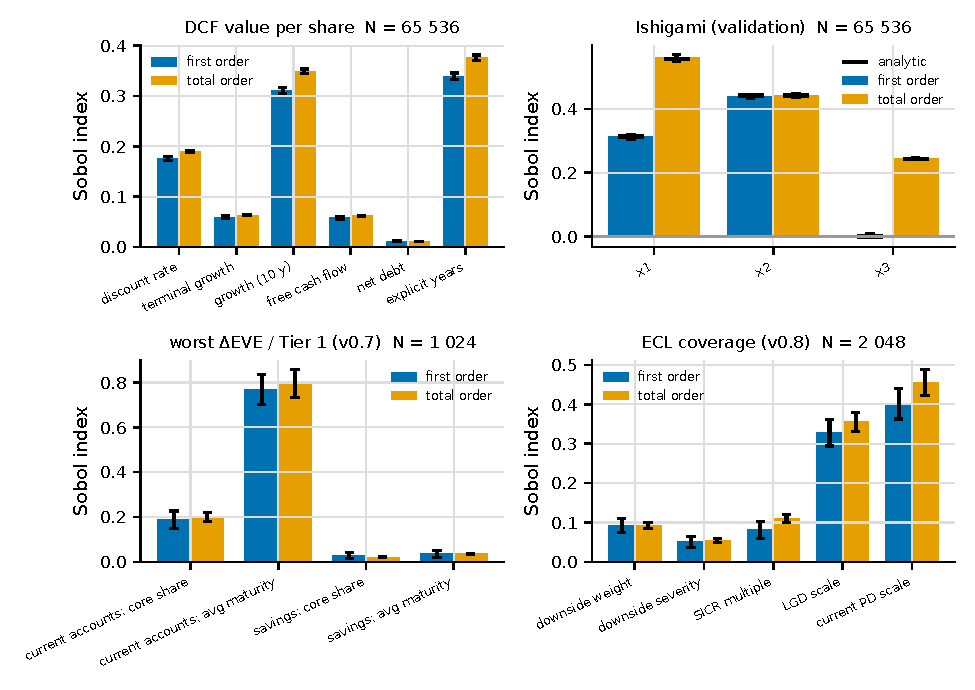
\includegraphics[width=0.66\linewidth]{figures/fig26_sobol.pdf}
\caption{Variance-based (Sobol) sensitivity indices: first order (the input alone) and total order (with all interactions), Saltelli sampling with the Jansen total-order estimator, error bars $\pm 1.96$ bootstrap se. Top left: the synthetic company's value per share over the six inputs and ranges of the tornado (the explicit period discrete uniform over 7--13 years). Top right: the Ishigami function, where the analytic indices (black marks) are known - a check of the estimator. Bottom: the same tool on the v0.7 bank (non-maturity-deposit assumptions) and on a v0.8 loan book (scenario weight and severity, SICR threshold, LGD and PD scaling).}
\label{fig:fig26_sobol}
\end{figure}
